\documentclass[11pt]{article}
\usepackage{amsmath}
\usepackage{amsfonts}
\usepackage{amsthm}
\usepackage{graphicx}
\usepackage{amssymb}
\usepackage{slashed}
\usepackage{listings}
\usepackage{color}

%----------------------------------------------------------------------------------------------------------------------------------------
% Defines various parameters for lstlisting for code snippets
\definecolor{dkgreen}{rgb}{0,0.6,0}
\definecolor{gray}{rgb}{0.5,0.5,0.5}
\definecolor{mauve}{rgb}{0.58,0,0.82}
\definecolor{highlight}{RGB}{255,251,204}

\lstset{frame=tb,
  language=R,
  backgroundcolor=\color{highlight},
  aboveskip=3mm,
  belowskip=3mm,
  showstringspaces=false,
  columns=flexible,
  basicstyle={\small\ttfamily},
  numbers=none,
  numberstyle=\tiny\color{gray},
  keywordstyle=\color{blue},
  commentstyle=\color{dkgreen},
  stringstyle=\color{mauve},
  breaklines=true,
  breakatwhitespace=true,
  tabsize=3}
%----------------------------------------------------------------------------------------------------------------------------------------

%----------------------------------------------------------------------------------------------------------------------------------------
% Set page geometry parameters
\textwidth = 6.5 in
\textheight = 8.5 in
\oddsidemargin = 0.0 in
\evensidemargin = 0.0 in
\topmargin = 0.0 in
\headheight = 0.0 in
\headsep = 0.5 in
\parskip = 0.2in
\parindent = 0.0in
%----------------------------------------------------------------------------------------------------------------------------------------

%----------------------------------------------------------------------------------------------------------------------------------------
%Defines macros for some mathematical tools.  Probably not useful here.
\providecommand{\abs}[1]{\lvert#1\rvert}
\providecommand{\norm}[1]{\lvert\lvert#1\rvert\lvert}
\providecommand{\inner}[2]{\langle#1 , #2\rangle}
\providecommand{\unionover}[3]{ {\underset{#1 \in #2}{\bigcup}} {#3}}
\providecommand{\intover}[3]{ {\underset{#1 \in #2}{\bigcap}} {#3}}

\providecommand{\code}[1]{{\color{red}\ttfamily #1}}
%----------------------------------------------------------------------------------------------------------------------------------------
\begin{document}
%----------------------------------------------------------------------------------------------------------------------------------------
%----------------------------------------------------------------------------------------------------------------------------------------

\section*{Chapter 2}
\begin{enumerate}
\subsection*{Conceptual}
\item  For each of parts (a) through (d), indicate whether we would generally expect the performance of a flexible statistical learning method to be better or worse than an inflexible method.  Justify your answer.
\begin{enumerate}
\item The sample size $n$ is extremely large, and the number of predictors $p$ is small.\\

An extremely large sample size will tend to mitigate overfitting issues.  Further having a small number of predictors will tend to decrease the variance of the decision boundary.  Thus a more flexible method is called for in this situation, as it will fit the data better and overfitting will be mitigated. 
\item The number of predictors $p$ is extremely large, and the number of observations $n$ is small.\\

With an extremely large number of predictors the variance of the decision boundary will be high.  Thus with a small sample size a flexible method will overfit the data.  Hence a less flexible method is called for.
\item The relationship between the predictors and response is highly non-linear.\\

Since the relationship is highly non-linear, a less flexible method will perform poorly due to it's high bias.  Thus a more flexible method is called for. 
\item The variance of the error terms, i.e. $\sigma^2=\text{Var}(\epsilon)$, is extremely high. \\

In this case the irreducible error is high and a highly flexible method will perform poorly due to overfitting the noise in the data.  Hence a less flexible method is called for.
\end{enumerate}

\item Explain whether each scenario is a classification or regression problem, and indicate whether we are most interested in inference or prediction.  Finally, provide $n$ and $p$.
\begin{enumerate}
\item We collect a set of data on the top 500 firms in the US.  For each firm we record profit, number of employees, industry and the CEO salary.  We are interested understanding which factors affect CEO salary.\\

This scenario is a regression problem, since the response variable is CEO salary which is a continuous quantity.  We are most interested in inference since we would like to know how the input variables affect the response variable, rather than just predicting CEO salary.  The predictors, $p$, here are profit, number of employees and industry.  In this example $n=500$ firms.
\item We are considering launching a new product and wish to know whether it will be a success of failure.  We collect data on 20 similar products that were previously launched.  For each product we have recorded whether it was a success or failure, price charged for the product, marketing budget, competition price and ten other variables.\\

This is a classification problem, since the response variable is success/failure which has discrete values.  We are most interested here in prediction since we wish only to find out if our new product will be successful rather than how the predictors contribute to its success.  The predictors are price charged for the product, marketing budget, competition price and the ten other variables.  In this example $n=20$ similar products.

\item We are interested in predicting the \% change in the US dollar in relation to the weekly changes in the world stock markets.  Hence we collect weekly data for all of 2012.  For each week we record the \% change in the dollar, the \% change in the US market, the \% change in the British market, and the \% change in the German market. \\

This is a regression problem, since the response variable is \% change in the US dollar which is real valued.  We are most interested here in prediciton, since we wish to predict the change in US dollar rather than analyze how equity markets affect it's value.  The predictors are the \% change in the US market, the \% change in the British market, and the \% change in the German market.  In this example $n=52$ weekly data points from 2012.
\end{enumerate}

\item We now revisit the bias-variance decomposition.
\begin{enumerate}
\item Provide a sketch of typical (squared) bias, variance, training error, test error, and Bayes (or irreducible) error curves on a single plot, as we go from less flexible statistical learning methods to more flexible approaches.  The $x$-axis should represent the amount of flexibility in the method, and the y-axis should represent the values for each curve.  There should be five curves.  Make sure to label each one.
\item Explain why each of the five curves has the shape displayed in part (a).
\end{enumerate}

\item You will now think of some real-life applications for statistical learning.
\begin{enumerate}
\item Describe three real-life applications in which classification might be useful.  Describe the response, as well as the predictors.  Is the goal of each application inference or prediction? Explain your answer.
\begin{enumerate}
\item Cancer Detection - Given attributes of a tumor (i.e. size, color, tissue density, etc.) predict whether the tumor is malignant or not.  This is a prediction problem since we wish only to predict whether the tumor is malignant or not, rather than how the factors affect malignancy. 
\item Credit Risk - Given various attributes of a company (i.e. debt, interest rate, stock price, market capitalization, revenue, profit, sector, dividend payment, etc.) predict whether the company will default.  As phrased, this is a prediction problem since we wish only to forecast a default.  However, the inference problem of how a companies attributes affect its default risk is also an interesting problem.
\item Direct Marketing - Given input variables such as customer purchase history, time of day, day of week, wording of e-mail, etc.  predict whether a customer will click on a link in an e-mail.  This is most fruitfully viewed as a inference problem, since we wish to optimize the time of day, wording, etc. of our e-mail campaign to maximize click-through-rate.
\end{enumerate}

\item Describe three real-life applications in which regression might be useful.  Describe the response, as well as the predictors.  Is the goal of each application inference or prediction? Explain your answer.
\begin{enumerate}
\item Real Estate - Given the attributes of a house (i.e. sq. footage, number of bedrooms, number of bathrooms, location, school district, offset, etc.) predict the selling price of the house.  This is a prediction problem since we wish to forecast the selling price of the house.
\item IPO Valuation - Given the attributes of a company and market (i.e. debt, revenue, profit, index levels, interest rate, CPI, $\alpha$, etc.) predict an appropriate initial offering price.  This is a prediction problem since we wish only to fix the appropriate price.  The inference problem, however,  is also interesting since a company will wish to maximize this initial price and so will wish to know what is the optimal market in which to offer.
\item  Life Insurance - Given the attributes of an individual (i.e. age, health, ethnicity, marital status, etc.) predict the individuals life expectancy.  This is a prediction problem. 
\end{enumerate}

\item  Describe three real-life applications in which cluster analysis might be useful.
\begin{enumerate}
\item Market Segmentation - Given a database of customer data cluster the customers into meaningful market segments.  This is an inference problem as we wish to infer how our customers clump into market segments.
\item Recommendation - Given a database of user and movie rating data predict a users rating of a movie based on the ratings of similar users.  This is a prediction problem, as we wish to predict a users rating of a given movie.
\item Anomaly Detection - From the observable properties of a battery (i.e. operating temperature,  voltage, current, charge time, ripple, etc.) determine if the battery is anomalous (and hence likely defective) or not.  This is a prediction problem. 
\end{enumerate}
\end{enumerate}

\item What are the advantages and disadvantages of a very flexible (versus a less flexible) approach for regression or classification?  Under what circumstances might a more flexible approach be preferred to a less flexible approach?  When might a less flexible approach be preferred?\\

The advantage of a very flexible learning method for regression and classification problems is that they are capable of accurately fitting highly nonlinear relationships between the predictors and response variable.  They also do not require an a priori knowledge of these nonlinearities.  The disadvantage of a highly flexible method is that they are prone to overfit the data.  More flexible methods also generally fit models which are more difficult to interpret.  A more flexible method is preferred when we have a prediction problem, and hence are not concerned with interpreting our model, a nonlinear relationship between the predictors and the response variable and/or enough data to mitigate overfitting.  A less flexible approach might be preferred if we wish to use our model to infer the relationship between the predictors and response, as the less flexible model will be more easily interpreted. A less flexible approach is also called for if we don't have a lot of data or find that a more flexible method has too high variance.    

\item Describe the differences between a parametric and a non-parametric statistical learning approach.  What are the advantages of a parametric approach to regression or classification (as opposed to a non-parametric approach)?  What are the disadvantages?\\

A parametric statistical learning methods makes an assumption about the form of $f$, which reduces the regression or classification problem to the problem of estimating the specific parameters of the assumed form of $f$.  A non-parametric method does not make an explicit assumption about the form of $f$, and instead seeks to select $f$ from some large class of functions.  Since a parametric methods reduce the problem to estimating a (small) number of parameters they can estimate $f$ accurately with fewer data.  However the assumed form may be too simple and so parametric methods may suffer from high bias.  Non-parametric methods avoid bias by not making an assumption about the form of the function, however they may suffer from high variance and a large data set is required for them to fit $f$ accurately. 

\item The table below provides a training data set containing six observations, three predictors, and one qualitative response variable.

\begin{center}
    \begin{tabular}{l|rrrl}
      \hline
      Obs. & $X_1$ & $X_2$ & $X_3$ & $Y$\\
      \hline
       1 &  0 & 3 & 0 & Red\\
       2 &  2 & 0 & 0 & Red\\
       3 &  0 & 1 & 3 & Red\\
       4 &  0 & 1 & 2 & Green\\
       5 & $-1$ & 0 & 1 & Green\\
       6 &  1 & 1 & 1 & Red\\
       \hline
    \end{tabular}
\end{center}

Suppose we wish to use this data set to make a prediction for $Y$ when $X_1=X_2=X_3=0$ using $K$-nearest neighbors.
\begin{enumerate}
\item Compute the Euclidean distance between each observation and the test point, $X_1=X_2=X_3=0$.\\

Let $X$ denote the observation $X_1=X_2=X_3=0$ and $X^i$ denote the $i$th training observation.  Then,
\begin{description}
\item $\norm{X-X_1}_2=3$
\item $\norm{X-X_2}_2=2$
\item $\norm{X-X_3}_2=\sqrt{10}$
\item $\norm{X-X_4}_2=\sqrt{5}$
\item $\norm{X-X_5}_2=\sqrt{2}$
\item $\norm{X-X_6}_2=\sqrt{3}$
\end{description}

\item What is our prediction with $K=1$? Why?\\

Note that observation 5 is the closest to $X$, so we predict that $X$ will produce the same response as $X^5$.  Thus we predict Green.
\item What is our prediction with $K=3$? Why?

Note that observations $5, 6$ and $2$ are the three nearest points to $X$.  Thus we estimate a probability of $\frac{2}{3}$ that $X$ should be Red and $\frac{1}{3}$ that $X$ should be Green.  Hence we predict Red.
\item If the Bayes decision boundary in this problem is highly non-linear, then would we expect the best value for $K$ to be large or small? Why?\\

In $K$-nearest neighbors, small values of $K$ produce low bias and high variance and large values of $K$ produce high bias and low variance.  Thus if the Bayes decision boundary is highly non-linear we should use a smaller value of $K$ to gain the flexibility to fit this non-linear boundary.
\end{enumerate}



\subsection*{Applied}
\item This exercise relates to the \code{College} data set, which can be found in the file \code{College.csv}.  It contains a number of variables for 777 different universities and colleges in the US.  Before reading the data into \code{R}, it can be viewed in Excel or a text editor.
\begin{enumerate}
\item Use the \code{read.csv()} function to read the data into \code{R}.  Call the loaded data \code{college}.  Make sure that you have the directory set to the correct location for the data.
\item Look at the data using the \code{fix()} function.  You should notice that the first column is just the name of each university.  We don't really want \code{R} to treat this as data.  However, it may be handy to have these names for later.  Try the following commands:

\begin{lstlisting}
> rownames(college)=college[,1]
> fix(college)
\end{lstlisting}

Now you should see that the first data column is \code{Private}.  Note that another column labeled \code{row.names} now appears before the \code{Private} column.  However, this is not a data columnbut rather the name that \code{R} is giving each row.

\item\begin{enumerate}
\item Use the \code{summary()} function to produce a numerical summary of the variables in the data set.
\item Use the \code{pairs()} function to produce a scatterplot matrix of the first ten columns or variables of the data.  Recall that you can reference the first ten columns of a matrix \code{A} using \code{A[,1:10]}.

\begin{lstlisting}
> summary(college[,1:10])
 Private        Apps           Accept          Enroll       Top10perc    
 No :212   Min.   :   81   Min.   :   72   Min.   :  35   Min.   : 1.00  
 Yes:565   1st Qu.:  776   1st Qu.:  604   1st Qu.: 242   1st Qu.:15.00  
           Median : 1558   Median : 1110   Median : 434   Median :23.00  
           Mean   : 3002   Mean   : 2019   Mean   : 780   Mean   :27.56  
           3rd Qu.: 3624   3rd Qu.: 2424   3rd Qu.: 902   3rd Qu.:35.00  
           Max.   :48094   Max.   :26330   Max.   :6392   Max.   :96.00
  \end{lstlisting}         
           
  \begin{lstlisting}           
   Top25perc      F.Undergrad     P.Undergrad         Outstate    
 Min.   :  9.0   Min.   :  139   Min.   :    1.0   Min.   : 2340  
 1st Qu.: 41.0   1st Qu.:  992   1st Qu.:   95.0   1st Qu.: 7320  
 Median : 54.0   Median : 1707   Median :  353.0   Median : 9990  
 Mean   : 55.8   Mean   : 3700   Mean   :  855.3   Mean   :10441  
 3rd Qu.: 69.0   3rd Qu.: 4005   3rd Qu.:  967.0   3rd Qu.:12925  
 Max.   :100.0   Max.   :31643   Max.   :21836.0   Max.   :21700  
   Room.Board  
 Min.   :1780  
 1st Qu.:3597  
 Median :4200  
 Mean   :4358  
 3rd Qu.:5050  
 Max.   :8124  
\end{lstlisting}

\item Use the \code{plot()} function to produce side-by-side boxplots of \code{Outstate} versus \code{Private}.

\begin{lstlisting}
> plot(college$Private, college$Outstate, xlab="Private", ylab="Outstate", main="Outstate vs. Private")
\end{lstlisting}
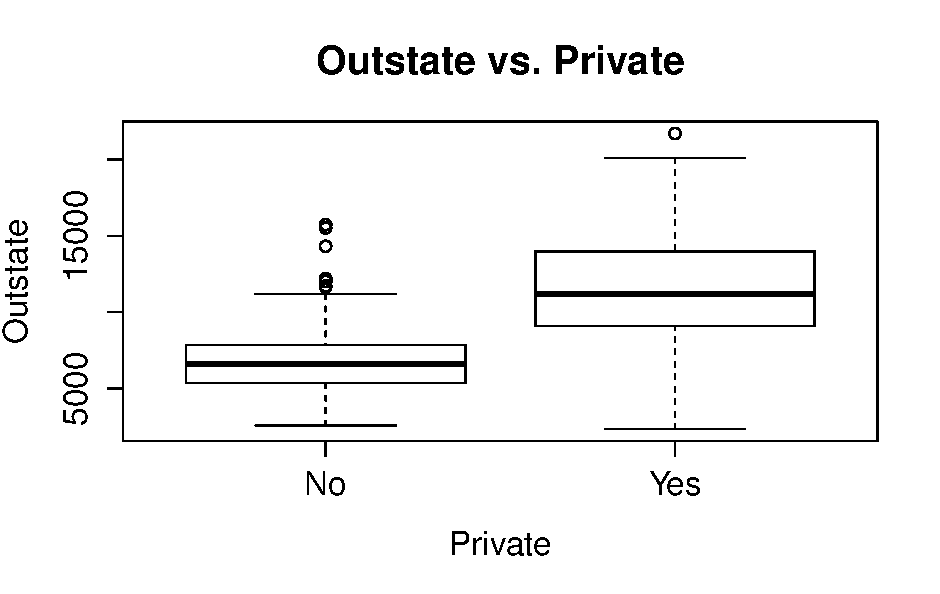
\includegraphics[scale = .9]{plot1.pdf}

\item Create a new qualitative variable, called \code{Elite}, by binning the \code{Top10perc} variable.  We are going to divide universities into two groups based on whether or not the proportion of students coming from top 10\% of their high school classes exceeds 50\%.

\begin{lstlisting}
> Elite = rep("No", nrow(college))
> Elite[college$Top10perc > 50]="Yes"
> Elite = as.factor(Elite)
> college = data.frame(college, Elite)
\end{lstlisting}

Use the \code{summary()} function to see how many elite universities there are.  Now use the \code{plot()} function to produce side-by-side boxplots of \code{Outstate} versus \code{Elite}.

\begin{lstlisting}
> summary(college$Elite)
 No Yes 
699  78 
\end{lstlisting}

\begin{lstlisting}
> plot(college$Elite, college$Outstate, main="Outstate vs. Elite", xlab = "Elite", ylab = "Outstate")
\end{lstlisting}
\begin{center}
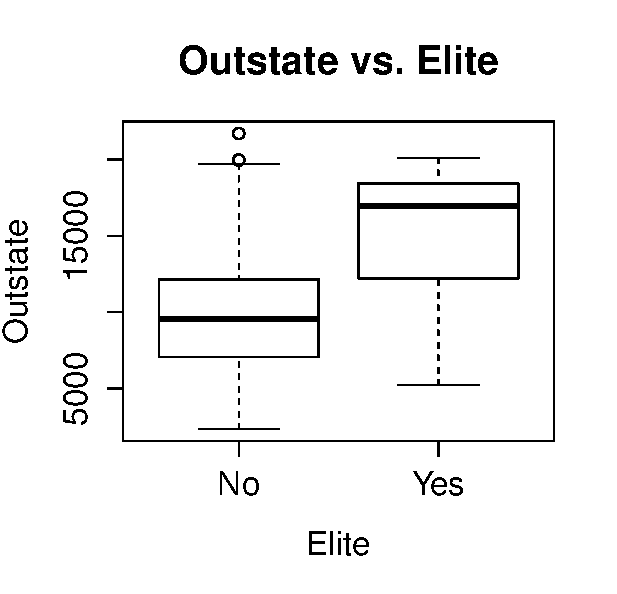
\includegraphics{plot2.pdf}
\end{center}

\item Use the \code{hist()} function to produce some histograms with differing numbers of bins for a few of the quantitative variables.  You may find the command \code{par(mfrow=c(2,2))} useful:  it will divide the print window into four regions so that four plots may be made simultaneously.

\begin{lstlisting}
> par(mfrow=c(2,2))
> hist(college$Outstate, breaks=5, main="Outstate")
> hist(college$Outstate, breaks=10, main="Outstate")
> hist(college$Outstate, breaks=15, main="Outstate")
> hist(college$Outstate, breaks=20, main="Outstate")
\end{lstlisting}
\begin{center}
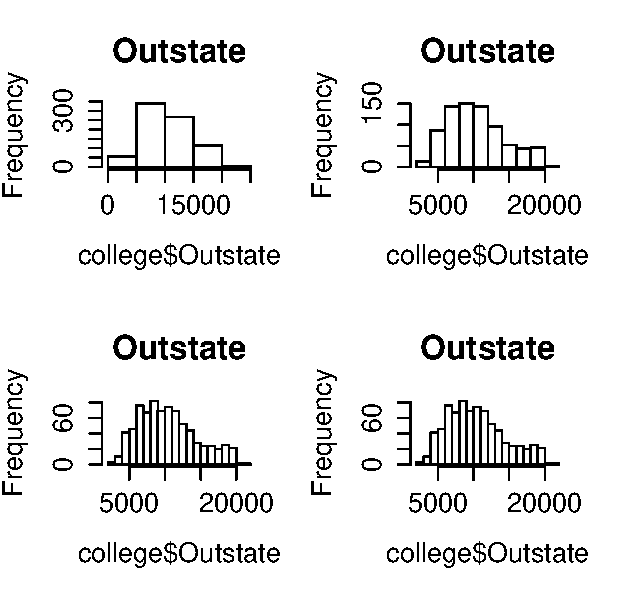
\includegraphics[scale=.9]{plot3.pdf}
\end{center}

\begin{lstlisting}
> hist(college$Expend, breaks=5, main="Expend")
> hist(college$Expend, breaks=10, main="Expend")
> hist(college$Expend, breaks=15, main="Expend")
> hist(college$Expend, breaks=20, main="Expend")
\end{lstlisting}
\begin{center}
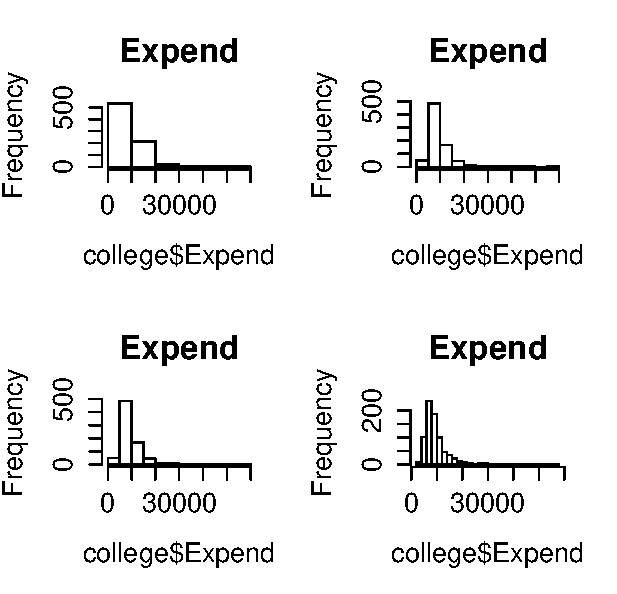
\includegraphics[scale=.9]{plot4.pdf}
\end{center}

\begin{lstlisting}
> hist(college$PhD, breaks=5, main="PhD")
> hist(college$PhD, breaks=10, main="PhD")
> hist(college$PhD, breaks=15, main="PhD")
> hist(college$PhD, breaks=20, main="PhD")
\end{lstlisting}
\begin{center}
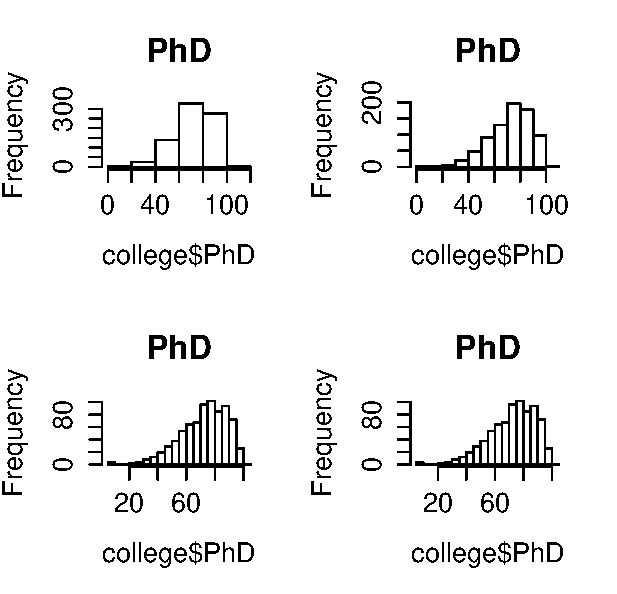
\includegraphics[scale=.8]{plot5.pdf}
\end{center}

\begin{lstlisting}
> hist(college$Grad.Rate, breaks=5, main="Grad.Rate")
> hist(college$Grad.Rate, breaks=10, main="Grad.Rate")
> hist(college$Grad.Rate, breaks=15, main="Grad.Rate")
> hist(college$Grad.Rate, breaks=20, main="Grad.Rate")
\end{lstlisting}
\begin{center}
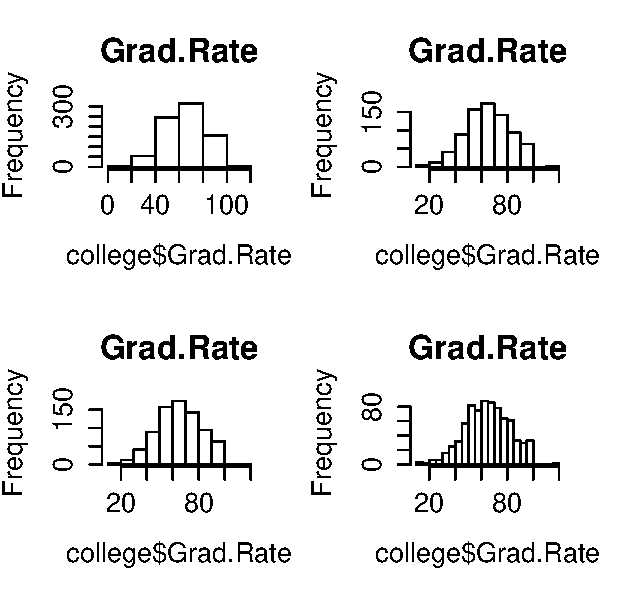
\includegraphics[scale=.8]{plot6.pdf}
\end{center}



\item Continue exploring the data, and provide a brief summary of what you discover.

\begin{lstlisting}
> plot(college$Top10perc, college$Grad.Rate)
> plot(college$S.F.Ratio, college$Grad.Rate)
> plot(college$Expend, college$Grad.Rate)
> plot(college$Outstate, college$Grad.Rate)
\end{lstlisting}
\begin{center}
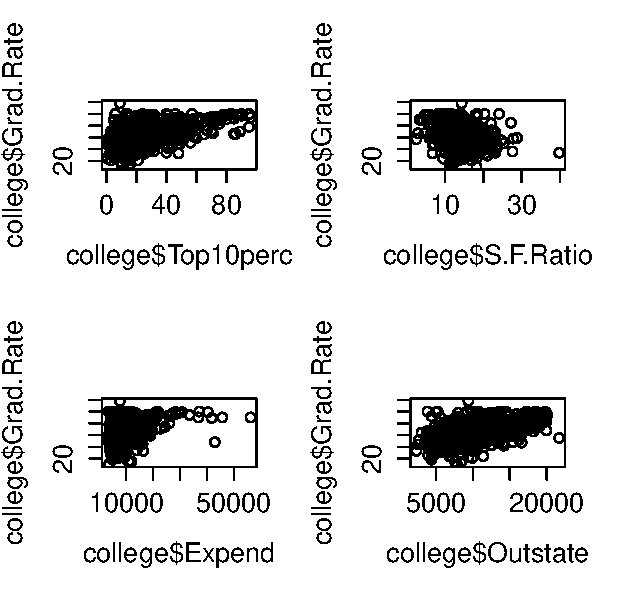
\includegraphics[scale=.9]{plot7.pdf}
\end{center}

More selective schools, schools with higher expenditures per student and colleges with higher tuition tend to have higher graduation rates.  Schools with lower student-to-faculty ratios tend to also have higher graduation rates.
\end{enumerate}
\end{enumerate}

\item This exercise involves the \code{Auto} data set studied in the lab.  Make sure that the missing values have been removed from the data.
\begin{enumerate}
\item Which of the predictors are quantitative, and which are qualitative?\\

The quantitative predictors are mpg, cylinders, displacement, horsepower, weight, acceleration and year.  The qualitative predictors are origin and name.
\item What is the range of each quantitative predictor?  You can answer this using the \code{range()} function.
\begin{lstlisting}
> sapply(Auto[,1:7], range)
      mpg cylinders displacement horsepower weight acceleration year
[1,]  9.0         3           68         46       1613          8.0    70
[2,] 46.6         8          455        230       5140         24.8    82
\end{lstlisting} 

\item What is the mean and standard deviation of each quantitative predictor?
\begin{lstlisting}
> sapply(Auto[,1:7], mean)
   mpg    cylinders displacement   horsepower       weight acceleration         year 
23.445918     5.471939   194.411990   104.469388  2977.584184    15.541327    75.979592 
> sapply(Auto[,1:7], sd)
   mpg    cylinders displacement   horsepower       weight acceleration         year 
7.805007     1.705783   104.644004    38.491160   849.402560     2.758864     3.683737 
\end{lstlisting}

\item Now remove the $10$th through $85$th observations.  What is the range, mean and standard deviation of each predictor in the subset of the data that remains?
\begin{lstlisting}
> trimmedAuto=Auto[-seq(10,85),]
> sapply(trimmedAuto[,1:7], range)
      mpg cylinders displacement horsepower weight acceleration year
[1,] 11.0         3           68         46       1649          8.5   70
[2,] 46.6         8          455        230       4997         24.8   82
> sapply(trimmedAuto[,1:7], mean)
  mpg    cylinders displacement   horsepower       weight acceleration         year 
24.404430     5.373418   187.240506   100.721519  2935.971519    15.726899    77.145570 
> sapply(trimmedAuto[,1:7], sd)
   mpg    cylinders displacement   horsepower       weight acceleration         year 
7.867283     1.654179    99.678367    35.708853   811.300208     2.693721     3.106217
\end{lstlisting}

\item Using the full data set, investigate the predictors graphically, using scatterplots or other tools of your choice.  Create some plots highlighting the relationships among the predictors.  Comment on your findings.
\begin{lstlisting}
> pairs(Auto[c(1,3,4,5,7)])
\end{lstlisting}
\begin{center}
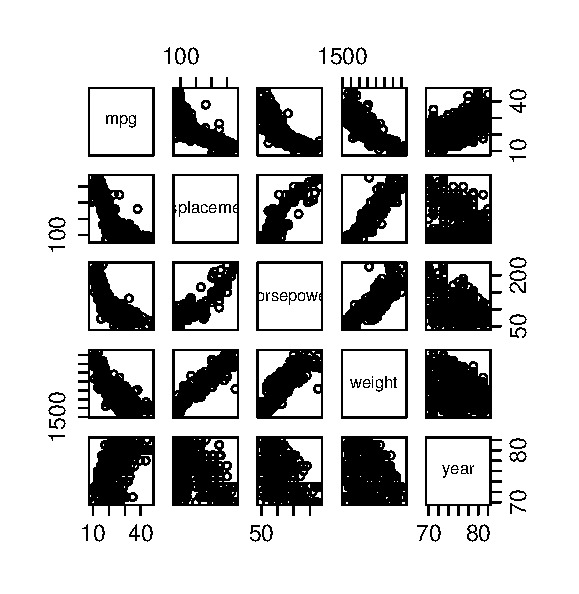
\includegraphics[scale=1.75]{plot8.pdf}
\end{center}

Displacement, horsepower and weight are all positively correlated with each other and negatively correlated with mpg.  The variance in mpg is large for a give year but year and mpg are positively correlated.  

\item Suppose that we wish to predict gas mileage on the basis of the other variables.  Do your plots suggest that any of the other variables might be useful in predicting \code{mpg}?  Justify your answer.\\

The above plots show that displacement, horsepower, weight and year are all correlated with mpg and hence will be useful in predicting mpg.  Also displacement, horsepower and weight are all strongly correlated with each other so including all of them may be redundant and not increase accuracy.
\end{enumerate}

\item This exercise involves the \code{Boston} housing data set.
\begin{enumerate}
\item To begin, load in the \code{Boston} data set.  The \code{Boston} data set is part of the \code{MASS} library in \code{R}.
\begin{lstlisting}
> library(MASS)
\end{lstlisting}
Now the data set is contained in the object \code(Boston).
\begin{lstlisting}
> Boston
\end{lstlisting}
Read about the data set:
\begin{lstlisting}
> ?Boston
\end{lstlisting}
How many rows are in the data set? How many columns? What do the rows and columns represent?
\begin{lstlisting}
> dim(Boston)
[1] 506  14
\end{lstlisting}
The data set contains 506 rows and 14 columns.
\item Make some pairwise scatterplots of the predictors (columns) in this data set.  Describe your findings.\\
\begin{lstlisting}
> plot(Boston$black, Boston$crim)
> plot(Boston$lstat, Boston$crim)
> plot(Boston$age, Boston$crim)
> plot(Boston$tax, Boston$ptratio)
\end{lstlisting}
\begin{center}
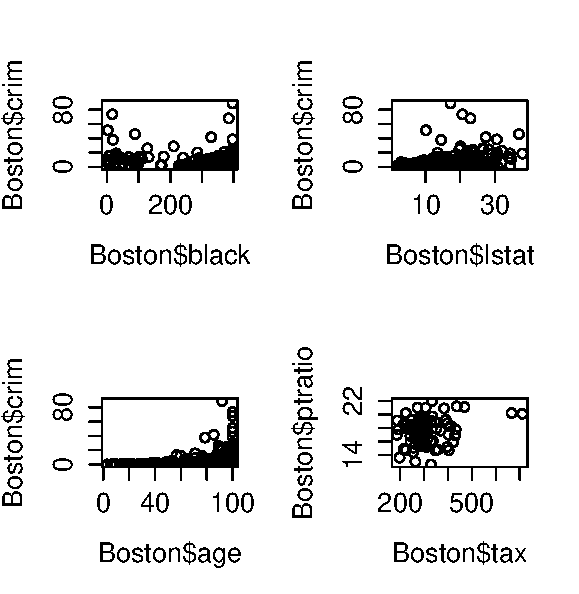
\includegraphics{plot9.pdf}
\end{center}

There does not seem to be a strong correlation between black and crime.  There is a positive correlation between both lstat and age with crime.  Surprisingly, there is not a strong correlation between tax and ptratio.
\item Are any of the predictors associated with per capita crime rate?  If so, explain the relationship.\\
As noted above, proportion of owner-occupied units built prior to 1940 and lower status of the population are both associated with per capita crime rate.  Additionally, median value of owner-occupied homes in \$1000s and weighted mean of distances to five Boston employment centers are associate with per capita crime rate.
\item Do any of the suburbs of Boston appear to have particularly high crime rates? Tax rates? Pupil-teacher ratios? Comment on the range of each predictor.
\begin{lstlisting}
> sapply(Boston, range)
      crim  zn indus chas   nox    rm   age     dis rad tax ptratio  black lstat medv
[1,]  0.00632   0  0.46    0 0.385 3.561   2.9  1.1296   1 187    12.6   0.32  1.73    5
[2,] 88.97620 100 27.74    1 0.871 8.780 100.0 12.1265  24 711    22.0 396.90 37.97   50
> hist(Boston$crim, breaks= 15, main= "Per Capita Crime")
> hist(Boston$tax, breaks= 15, main= "Tax")
> hist(Boston$ptratio, breaks= 15, main= "Pupil Teacher ratio")
\end{lstlisting}
\begin{center}
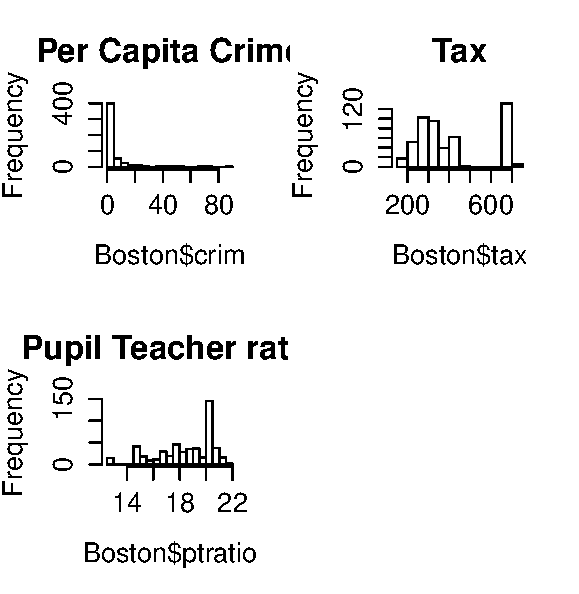
\includegraphics[scale=1.25]{plot10.pdf}
\end{center}

The histogram of per capita crime has an extremely long tail, with almost all suburbs having a rate lest than 10, but one with a rate of $89\%$.  The distribution of tax is bimodal with many observations near 300 and a large spike near 700.  The teacher-pupil ratio histogram shows two suburbs with extremely low ratios near 12.6 while all other obsevations are higher than 14 with a large spike at 20.

\item How many of the suburbs in this data set bound the Charles river?
\begin{lstlisting}
> dim(subset(Boston, chas==1))
[1] 35 14
\end{lstlisting}

There are 35 suburbs bounding the Charles.
\item What is the median pupil-teacher ratio among the towns in this data set?
\begin{lstlisting}
> median(Boston$ptratio)
[1] 19.05
\end{lstlisting}
\item Which suburb of Boston has lowest median value of owner occupied homes?  What are the values of the other predictors for that suburb, and how do those values compare to the overall ranges for those predictors?  Comment on your findings.
\begin{lstlisting}
> subset(Boston, Boston$medv == min(Boston$medv))
       crim zn indus chas   nox    rm age    dis rad tax ptratio  black lstat medv
399 38.3518  0  18.1    0 0.693 5.453 100 1.4896  24 666    20.2 396.90 30.59    5
406 67.9208  0  18.1    0 0.693 5.683 100 1.4254  24 666    20.2 384.97 22.98    5
\end{lstlisting}
These are the oldest suburbs with high tax rates, low distances to employment centers and have relatively high crime rates.

\item In this data set, how many of the suburbs average more than seven rooms per dwelling?  More than eight rooms per dwelling? Comment on the suburbs that average more than eight rooms per dwelling.
\begin{lstlisting}
> dim(subset(Boston, rm>7))
[1] 64 14
> dim(subset(Boston, rm>8))
[1] 13 14
> subset(Boston, rm>8)
       crim zn indus chas    nox    rm  age    dis rad tax ptratio  black lstat medv
98  0.12083  0  2.89    0 0.4450 8.069 76.0 3.4952   2 276    18.0 396.90  4.21 38.7
164 1.51902  0 19.58    1 0.6050 8.375 93.9 2.1620   5 403    14.7 388.45  3.32 50.0
205 0.02009 95  2.68    0 0.4161 8.034 31.9 5.1180   4 224    14.7 390.55  2.88 50.0
225 0.31533  0  6.20    0 0.5040 8.266 78.3 2.8944   8 307    17.4 385.05  4.14 44.8
226 0.52693  0  6.20    0 0.5040 8.725 83.0 2.8944   8 307    17.4 382.00  4.63 50.0
227 0.38214  0  6.20    0 0.5040 8.040 86.5 3.2157   8 307    17.4 387.38  3.13 37.6
233 0.57529  0  6.20    0 0.5070 8.337 73.3 3.8384   8 307    17.4 385.91  2.47 41.7
234 0.33147  0  6.20    0 0.5070 8.247 70.4 3.6519   8 307    17.4 378.95  3.95 48.3
254 0.36894 22  5.86    0 0.4310 8.259  8.4 8.9067   7 330    19.1 396.90  3.54 42.8
258 0.61154 20  3.97    0 0.6470 8.704 86.9 1.8010   5 264    13.0 389.70  5.12 50.0
263 0.52014 20  3.97    0 0.6470 8.398 91.5 2.2885   5 264    13.0 386.86  5.91 48.8
268 0.57834 20  3.97    0 0.5750 8.297 67.0 2.4216   5 264    13.0 384.54  7.44 50.0
365 3.47428  0 18.10    1 0.7180 8.780 82.9 1.9047  24 666    20.2 354.55  5.29 21.9
\end{lstlisting}
\end{enumerate}
There are 64 suburbs which average more than seven rooms per dwelling and 13 suburbs which average more than eight rooms per dwelling.  These suburbs have relatively low crime, and low lower status populations and higher median property value.











\end{enumerate}
%----------------------------------------------------------------------------------------------------------------------------------------
\end{document}